
\subsection{Ejercicios}
\begin{itemize}
 
\item \textbf{Ejercicio 6}  Programar un tipo de tarea TaskBatch que reciba dos parametros: total cpu y
cant bloqueos. Una tarea de este tipo debera realizar cant bloqueos llamadas bloqueantes, en
momentos elegidos pseudoaleatoriamente. En cada tal ocasion, la tarea debera permanecer
bloqueada durante exactamente un (1) ciclo de reloj. El tiempo de CPU total que utilice una
tarea TaskBatch debera ser de total cpu ciclos de reloj (incluyendo el tiempo utilizado para
lanzar las llamadas bloqueantes; no ası el tiempo en que la tarea permanezca bloqueada).

\item \textbf{Ejercicio 7} Elegir al menos dos metricas diferentes, definirlas y explicar la semantica de
su definicion. Diseñar un lote de tareas TaskBatch, todas ellas con igual uso de CPU, pero
con diversas cantidades de bloqueos. Simular este lote utilizando el algoritmo SchedRR y una
variedad apropiada de valores de quantum. Mantener fijo en un (1) ciclo de reloj el costo de
cambio de contexto y dos (2) ciclos el de migracion. Deben variar la cantidad de nucleos de
procesamiento. Para cada una de las metricas elegidas, concluir cual es el valor optimo de
quantum a los efectos de dicha metrica.

\item \textbf{Ejercicio 8} Implemente un scheduler Round-Robin que no permita la migracion de procesos
entre nucleos (SchedRR2). La asignacion de CPU se debe realizar en el momento en que se produce la carga 
de un proceso (load). El nucleo correspondiente a un nuevo proceso sera aquel
con menor cantidad de procesos activos totales (RUNNING + BLOCKED + READY). Diseñe y realice un conjunto 
de experimentos que permita evaluar comparativamente las dos implementaciones de Round-Robin.

\item \textbf{Ejercicio 9} Disenar un lote de tareas cuyo scheduling no sea factible para el algoritmo de
prioridades fijas pero sı para el algoritmo de prioridades dinamicas.

\item \textbf{Ejercicio 10} Disenar un lote de tareas, cuyo scheduling sı sea factible con el algoritmo de
prioridades fijas, donde se observe un mejor uso del CPU por parte del algoritmo de prioridades
dinamicas.
\end{itemize}
\subsection{Resultados y Conclusiones}

\subsubsection[Resolución Ejercicio 6]{Ejercicio 6}

\indent Al igual que con la tarea TaskConsola, mencionaremos nuestro implementación y acontinuación de la misma 
explicaremos ciertos puntos de la misma.\\
 \begin{verbatim}
                       void TaskBatch(int pid, vector<int> params) {
                            int total_cpu = params[0];
                            int cant_bloqueos = params[1];
                            srand(time(NULL));
                            vector<bool> uso = vector<bool>(total_cpu);
                            for(int i=0;i<(int)uso.size();i++) 
                               uso[i] = false;
	                       for(int i=0;i<cant_bloqueos;i++) {
                                   int j = rand()%(uso.size());
                                   if(!uso[j])
                                      uso[j] = true;
                                   else
                                      i--; 
                                   }
                            for(int i=0;i<(int)uso.size();i++) {
                                if( uso[i] )
                                    uso_IO(pid,1); 
                                else
                                    uso_CPU(pid, 1); 
                               }
                            }
 \end{verbatim}

 \indent Para este tipo de tarea, creamos un vector de tamaño igual a $total_cpu$ el cual tendra bool, ya sea true o false
 dependiendo del uso que se le de dentro de la tarea, ya sea uso\_IO o uso\_CPU. En caso de ser uso\_IO sera true, y sino false.\\
 Luego, utilizaremos un ciclo que ira desde 0 hasta el tamaño del vector y dependiendo el valor booleano, usará la funciones
 dadas por la catedra uso\_IO o uso\_CPU.\\
 
 \subsubsection[Resolución Ejercicio 7]{Ejercicio 7}
 Las métricas elegidas fueron:
\begin{itemize}
 \item \textbf{Turnaround}: Es el intervalo de tiempo desde que un proceso es cargado hasta que este finaliza su ejecución.
 \item \textbf{Waiting Time}: Es la suma de los intervalos de tiempo que un proceso estuvo en la cola de procesos $ready$.
\end{itemize}

\indent \indent Como las tareas TaskBatch se bloquean pseudoaleatoriamente, 
para obtener datos relevantes tomamos un promedio de las mediciones.\\
\indent A la hora de encarar la experimentación, lo que realizamos trabajar con
varios quantum distintos para poder obtener una mejor apreciacion 
del efecto del $quantum$ en la ejecución de este tipo de tareas. 

\indent A partir de este resultado, desarrollamos los siguientes gráficos de turnaround time 
en función del quantum, utilizando 2 y 3 núcleos

\indent Luego de realizar mediciones con distintos $quantum$,
tomamos la decisión de trabajar con los mismos $quantum$ para cada nucleo
al trabajar con más de 1 core. Igualmente, mostraremos a continuacion un grafico
ejemplificando la diferencia que se produce al trabajar con distintos $quantums$ por
core.\\

\begin{center}
    	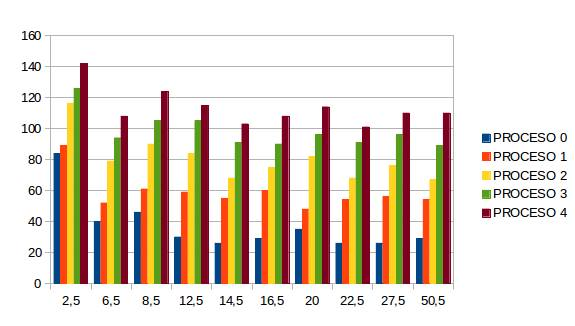
\includegraphics[width=1\textwidth]{./EJ7/turnarounddistquan.png}
	{Turnaround - 2 core - Prueba Quantum distintos por Core}\\
	{$Eje X = Quantum; $\\$ Eje Y = Tiempo$}\\
 \end{center}

\indent Al realizar este gráfico y varias mediciones con distintos $quantum$ 
por core, observamos que no eran mediciones rigurosas, 
ya que una proceso podria estar corriendo con distintos tiempos por la
migracion de procesos por core.\\

 \indent Por consiguiente, al trabajar con las nuevas mediciones, 
 concluimos con 2 hipotesis:
 
 \begin{itemize}
  \item Con 2 nucleos las mediciones de tiempo tienden a estabilizarse a partir de un $quantum$ igual a 9.
  \item Con 3 nucleos las mediciones de tiempo tienden a estabilizarse a partir de un $quantum$ igual a 11.
 \end{itemize}
 \begin{center}
 \textbf{Turnaround Time} 
  \end{center}

 \begin{center}
 \textbf{2 Core}
 \end{center}
  A continuación se muestran los Diagramas de Gantt más relevantes:
  
  \begin{center}
    	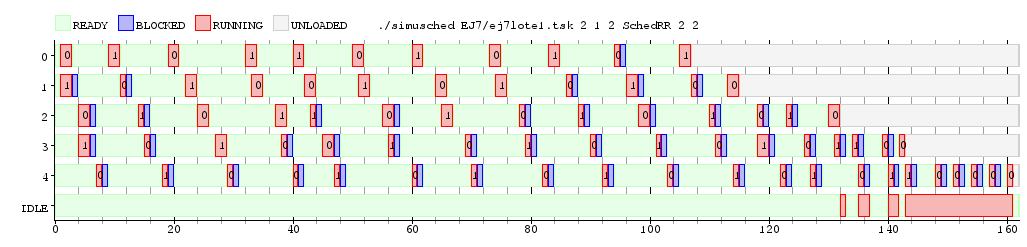
\includegraphics[width=450pt]{./EJ7/ej7tour2core1quan.png}
	{$Lote 1$ - Turnaround - 2 core - Quantum igual a 2}	
 \end{center}

   \begin{center}
    	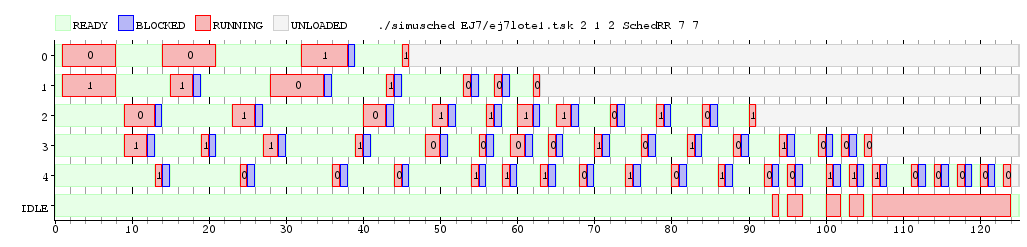
\includegraphics[width=450pt]{./EJ7/ej7tour2core3quan.png}
	{$Lote 1$ - Turnaround - 2 core - Quantum igual a 7}	
 \end{center}
 
 
 \indent La performance empieza a mejorar a medida que el $quantum$ aumenta.
 
   \begin{center}
    	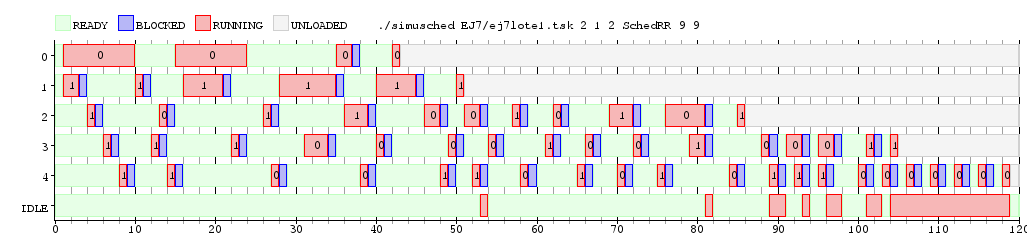
\includegraphics[width=450pt]{./EJ7/ej7tour2core4quan.png}
	{$Lote 1$ - Turnaround - 2 core - Quantum igual a 9}	
 \end{center}

  
   \indent La performance sigue mejorando,a partir de este valor, el desempeño 
   comienza a estabilizarse, como muestran los siguiente dos gráficos. 
   
   Las pequeñas diferencias en los valores se deben a que este tipo de tarea presenta
   una pseudoaleatoridad notoria.\\
  
   \begin{center}
    	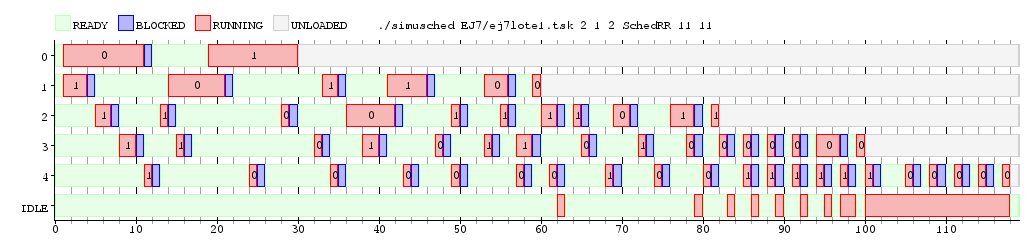
\includegraphics[width=450pt]{./EJ7/ej7tour2core5quan.png}
	{$Lote 1$ - Turnaround - 2 core - Quantum igual a 11}	
 \end{center}
 

    \begin{center}
    	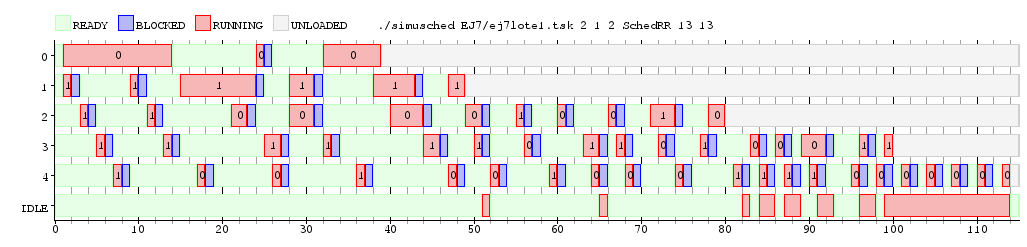
\includegraphics[width=450pt]{./EJ7/ej7tour2core8quan.png}
	{$Lote 1$ - Turnaround - 2 core - Quantum igual a 13}	
 \end{center}

 \indent Como mencionamos, las mediciones tienden a estabilizarse con un $quantum$ 
 igual a 9, pero la mejor performance obtenida es con un $quantum$ igual a 13,
 teniendo en cuenta como mencionamos la pseudoaleatoridad de este tipo de tarea.\\
 \indent Se puede observar en la primer figura que a pesar de trabajar con 2 cores, 
 al tener un quantum bajo (igual a 2)  el costo es alto.
  
   \begin{center}
    	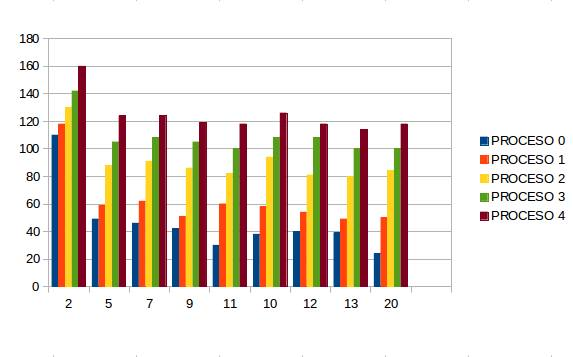
\includegraphics[width=1\textwidth]{./EJ7/tour2core.png}
	{Turnaround - 2 core}	\\
	{$Eje X = Quantum$\\$ Eje Y = Tiempo$}\\
 \end{center} 
 
 \begin{center}
  \textbf{Waiting Time}
 \end{center}

  \begin{center}
    	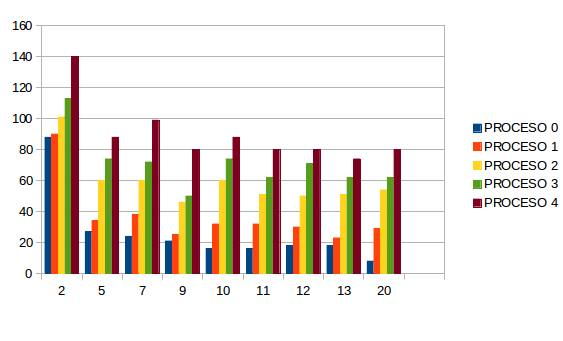
\includegraphics[width=1\textwidth]{./EJ7/waiting2core.jpg}
	{Waiting Time - 2 core}	\\
	{$Eje X = Quantum$\\$Eje Y = Tiempo$}\\
 \end{center} 
 
 \indent Con este tipo de metrica, se comienza a estabilizar a partir del $quantum$ igual
 a 5, obteniendo su mejor  performance con el $quantum$ igual a 13.\\
 
   \begin{center}
   \textbf{3 Core}
   \end{center}
   \indent A continuación, al igual que con 2 cores, mostraremos los resultados mas relevantes:
   
   \begin{center}
    	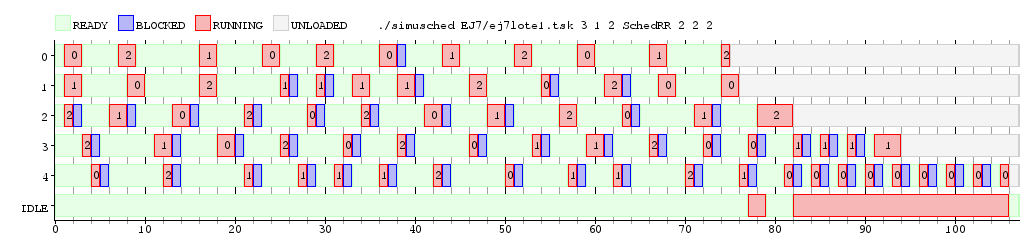
\includegraphics[width=450pt]{./EJ7/ej7tour3core1quan.png}
	{$Lote 1$ - Turnaround - 3 core - Quantum igual a 2}	
 \end{center}

 \indent Se observa que al tener otro core mas,a diferencia de con 2, 
 a pesar de estar con un $quantum$ bajo, la performance va en alto.\\ 
 
   \begin{center}
    	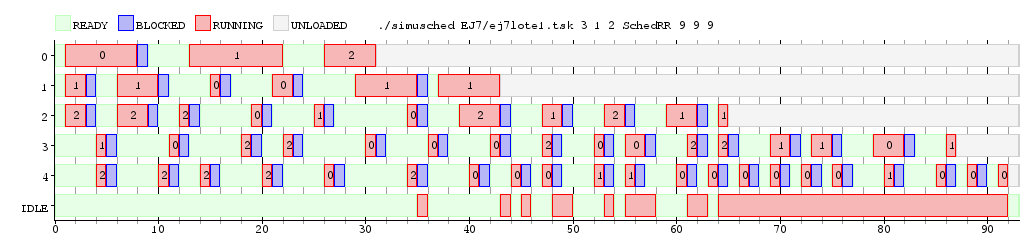
\includegraphics[width=450pt]{./EJ7/ej7tour3core4quan.png}
	{$Lote 1$ - Turnaround - 3 core - Quantum igual a 9}	
 \end{center}
 
 
 \indent La performance empieza a mejorar a medida que el $quantum$ aumenta.
 
   \begin{center}
    	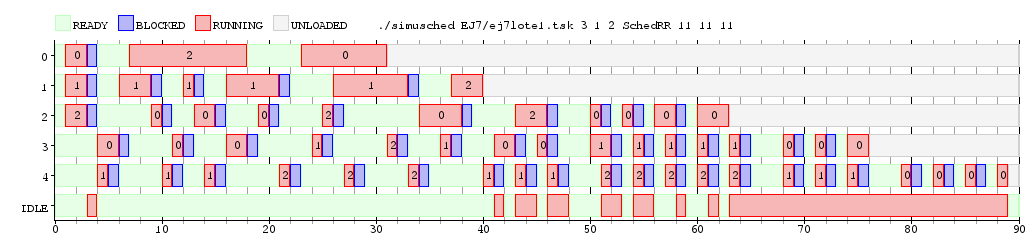
\includegraphics[width=450pt]{./EJ7/ej7tour3core5quan.png}
	{$Lote 1$ - Turnaround - 3 core - Quantum igual a 11}	
 \end{center}
  
   \begin{center}
    	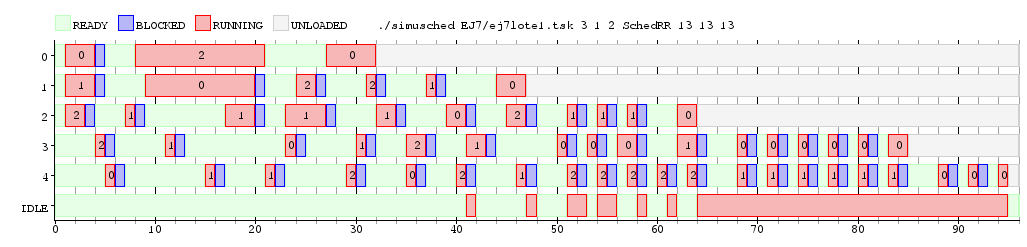
\includegraphics[width=450pt]{./EJ7/ej7tour7core6quan.png}
	{$Lote 1$ - Turnaround - 3 core - Quantum igual a 13}	
 \end{center}
 
 \begin{center}
    	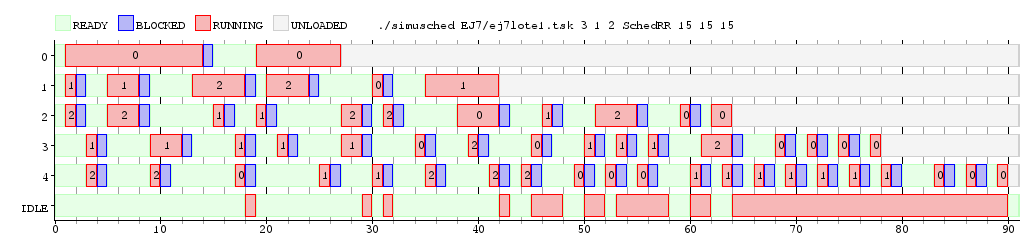
\includegraphics[width=450pt]{./EJ7/ej7tour8core6quan.png}
	{$Lote 1$ - Turnaround - 3 core - Quantum igual a 15}	
 \end{center}
 
 \indent A diferencia que en nuestra hipótesis conjeturada para con dos cores, 
 con un $quantum$ igual a 11 se obtiene la mejor  performance, 
 pero teniendo en cuenta el tipo de tarea con la 
 que se estuvo trabajando, a partir del $quantum$ igual a 9 ya se estabiliza notoriamente.\\
   
    \begin{center}
    	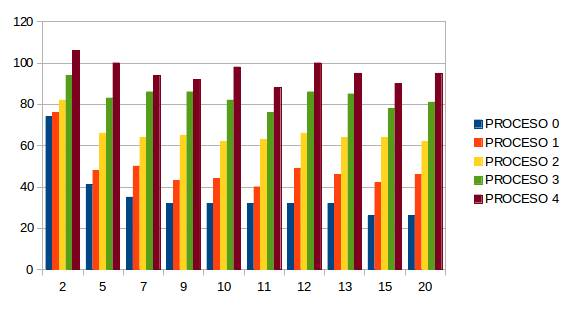
\includegraphics[width=1\textwidth]{./EJ7/tour3core.png}
	{Turnaround - 3 core}\\
	{$Eje X = Quantum $\\$ Eje Y = Tiempo$}\\
 \end{center} 
  
   \begin{center}
  \textbf{Waiting Time}
 \end{center}

  \begin{center}
    	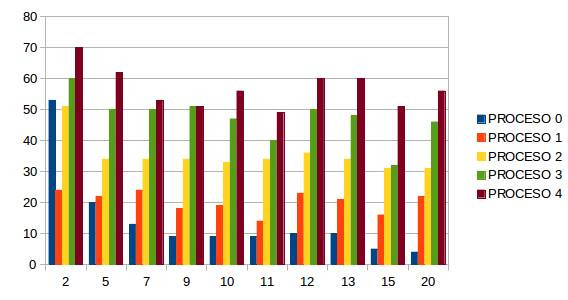
\includegraphics[width=1\textwidth]{./EJ7/waintin3core.jpg}
	{Waiting Time - 3 core}	\\
	{$Eje X = Quantum $\\$Eje Y = Tiempo$}\\
 \end{center} 
 
   \indent Con este tipo de metrica,se obteniene a diferencia de con Turnaround  
   su mejor performance con el $quantum$ igual a 15.\\
  
 \begin{center}
  \textbf{Conclusiones}
 \end{center}


\indent \indent La diferencia entre los valores de quantum entre los casos 
se puede presumir a que cada vez que agregamos un núcleo aumentamos 
la posibilidad de una migración de la tareas.\\
\indent \indent En todos lo casos se observa la influencia negativa que proviene 
de elegir un quantum con valores pequeños.\\
\indent \indent Agregar núcleos de procesamiento mejora significativamente 
la performance de acuerdo a la métricas con las que
trabajamos, al permitir más procesamiento en pararelo y disminuyendo 
los waiting time de las tareas.\\
\indent \indent  Fijada una cantidad de núcleos puntual, aumentar el valor del
quantum también mejora la performance, igualmente, como vimos, a partir de cierto valor 
de quantum, las mejoras en la performance tienden a estabilizarse y dejan de ser 
muy significativas. 
Esto se produce a que las tareas con mas cantidad de bloqueos en 
algun momento dejan de consumir todo el quantum otorgado si este es aumentado en su valor. 
 
 
 
\subsubsection[Resolución Ejercicio 8]{Ejercicio 8}
La idea principal de esta nueva version de $Round-Robin$ se centraliza en que no permita migracion entre
cores, esto se basa principalmente en utilizar una cola para cada nucleo por separado, y en cada
cola respectiva se encolaran las tareas que fueron asignadas inicialmente a cada nucleo.\\
Para desarrollar este tipo de algoritmo, el cual denominaremos $RR2$, utilizamos estructuras
puntuales, enunciadas a continuacion:\\
\begin{itemize}
 \item Un vector $quantum$ y otro $quantumActual$, los cuales siguen cumpliendo la misma funcion que
 en Round-Robin 1.
 \item Un vector de colas denominado $colas$, en el cual la posicion $i$ encontraremos la cola correspondiente
 a ese nucleo de procesamiento.
 \item Un diccionario de $Bloqueados$, donde la clave contendra el numero de core, y en definicion
 la tareas bloqueadas de ese core. Esto nos beneficiara cuando haya que reubicarla en la cola de procesos ready.
 \item Un vector de enteros $cantidad$, que como la palabra lo define, tendra en cada posicion $i$ 
 la totalidad de las tareas, ya sea bloqueadas, activas o en estado ready que tiene asignado ese core, beneficiandonos
 la determinacion del nucleo al que se asignara la tarea al momento de cargarla.
\end{itemize}
Cuando se carga una tarea, previamente, se chequeara que core tiene menor cantidad de procesos totales asignados (
aqui es donde el vector $cantidad$ entra en juego). Una vez que se obtiene este nucleo, se agrega 
la tarea a la cola correspondiente y se actualiza la cantidad sumando una unidad.\\
\indent Al bloquearse un proceso, se define una nueva entrada en el diccionario $bloqueados$ con el
pid y el nucleo correspondiente. De esta forma, al desbloquearse, colocamos la tarea en la cola del core
correspondiente y eliminamos la entrada del diccionario. Así logramos resolver el inconveniente de la nula
migracion entre nucleos.\\
\indent Finalmente, cuando una tarea finaliza, la quitamos y descontamos una unidad a la posicion $i$ del vector
$cantidad$. Esta es la unica vez, en la cual se descuenta. Aunque una tarea se bloquee, la misma
seguira contando en el vector. De esta forma se cumplira, que las tareas son asignadas a los cores
con menor cantidad de tareas.\\
Luego de realizar dicha implementacion, en comparacion al Round-Robin original, hemos conjeturado 
las siguientes hipotesis:

\begin{enumerate}
 \item Dados un mismo lote de tareas y una misma configuracion del scheduler (mismos costo en cambio
de contexto y quantum) un unico nucleo de procesamiento, ambos algoritmos deben comportarse
de la misma manera.
\item Comportamiento menos eficiente en el RR2 con respecto al paralelismo, ya que al no permitir
migracion de nucleos este lo pierde.
\item Comportamiento mas eficiente en el RR2 con lotes de tareas que se bloquean un gran numero
de veces. Esto surge ya que el Round-Robin original, es mas proclive a realizar cambios de contexto con la posibilidad
de darse un cambio de core.
\end{enumerate}

Por consiguiente, procederemos a demostrar lo conjeturado.\\

Iniciando con nuestra primer conjetura:\\

\textbf{Dados un mismo lote de tareas y una misma configuracion del scheduler 
 (mismos costo en cambio de contexto y quantum)
un unico nucleo de procesamiento, ambos algoritmos deben comportarse
de la misma manera.}\\

Trabajando con el lote que mencionamos a continuacion:
    
    \begin{verbatim}
                                     TaskCPU 70
                                     TaskConsola 2 4 5
                                     TaskCPU 40
                                     TaskConsola 3 2 3
                                     TaskCPU 30
    \end{verbatim}

Utilizando un $quantum$ igual a 5 y un cambio de contexto igual a 1 obtuvimos 
resultados muy marcados, viendose notoriamente lo que queremos demostrar.\\

\begin{center}
    	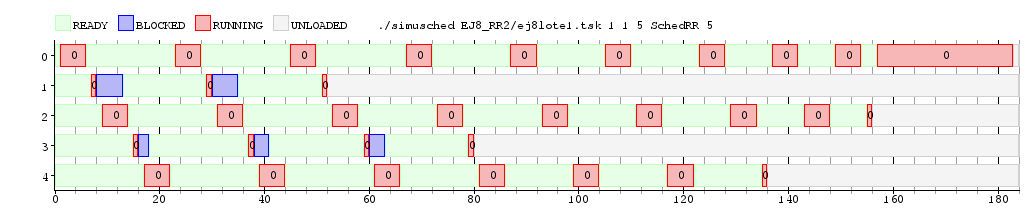
\includegraphics[width=450pt]{./EJ8_RR2/dif1corerr.png}
	{$Lote 1$ - Round Robin - 1 core - Quantum = 5 - cambio de contexto = 1}	
 \end{center}
 
 \begin{center}
    	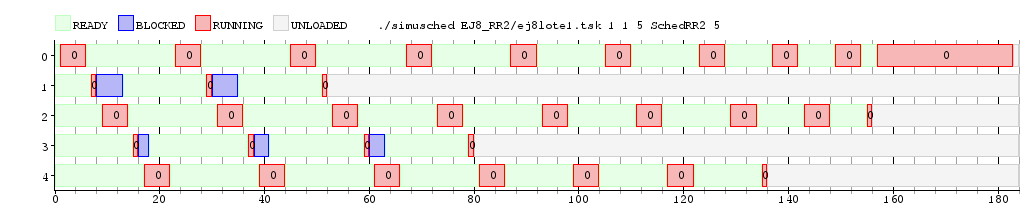
\includegraphics[width=450pt]{./EJ8_RR2/dif1corerr2.png}
	{$Lote 1$ - Round Robin 2 - 1 core - Quantum = 5 - cambio de contexto = 1}	
 \end{center}

Continuando con un lote distinto para ser mas precisos:

 \begin{verbatim}
                                     TaskCPU 70
                                     TaskConsola 5 6 7
                                     TaskCPU 40
                                     TaskConsola 10 9 8
                                     TaskCPU 30
 \end{verbatim}
 
Llegamos a lo siguiente:\\

 \begin{center}
    	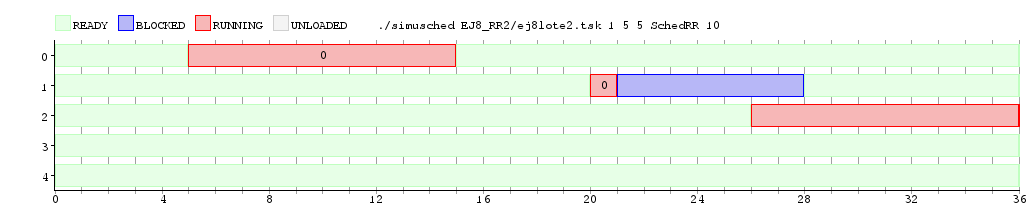
\includegraphics[width=450pt]{./EJ8_RR2/dif2corerr.png}
	{$Lote 2$ - Round Robin - 1 core - Quantum = 10 - cambio de contexto = 5}	
 \end{center}
 
 \begin{center}
    	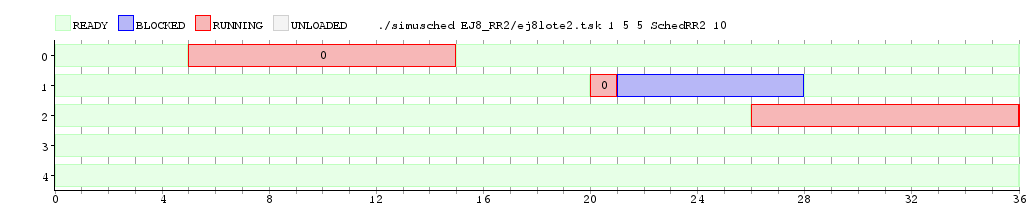
\includegraphics[width=450pt]{./EJ8_RR2/dif2corerr2.png}
	{$Lote 2$ - Round Robin 2 - 1 core - Quantum = 10 - cambio de contexto = 5}	
 \end{center}
 
 Viendose nuevamente, la igualdad que mencionamos. Hemos podido ver a su vez, que la unica
 forma en la que los resultados sean distintos con el mismo lote seria modificando o la
 cantidad de $quantum$ o la unidad de cambio de contexto entre uno y otro.\\
 
 Aqui, un ejemplo para mayor precision:\\
 
  \begin{center}
    	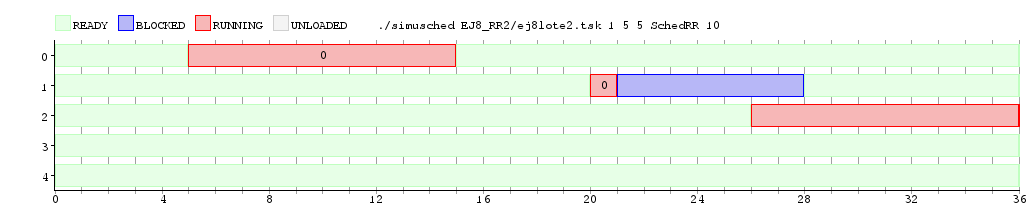
\includegraphics[width=450pt]{./EJ8_RR2/dif3corerr.png}
	{$Lote 2$ - Round Robin - 1 core - Quantum = 10 - cambio de contexto = 5}	
 \end{center}
 
 \begin{center}
    	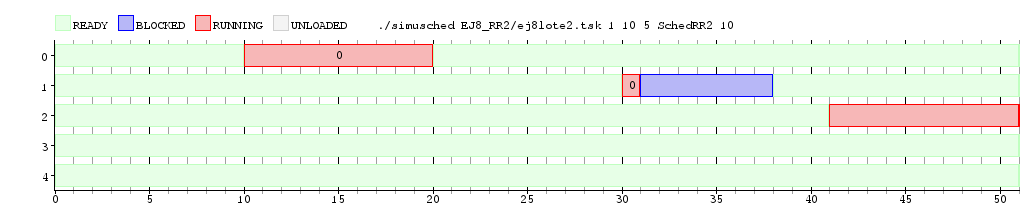
\includegraphics[width=450pt]{./EJ8_RR2/dif3corerr2.png}
	{$Lote 2$ - Round Robin 2 - 1 core - Quantum = 10 - cambio de contexto = 10}	
 \end{center}
 
 Concluimos entonces que, al trabajar con colas globales o no, utilizando un unico nucleo y
 mismo lote quantum y cambio de contexto, ambos schedulers se comportan de la misma
 manera.\\
 
 Procedemos a demostrar la segunda conjetura:\\
 
 \textbf{Comportamiento menos eficiente en el RR2 con respecto al paralelismo, ya que al no permitir
migracion de nucleos este lo pierde}\\

Para demostrar esta conjetura trabajamos con procesos que demanden mas uso del cpu como 
lo son las $taskCPU$\\

Un ejemplo de los lotes utilizados fue el siguiente:\\

\begin{verbatim}
                                     TaskCPU 40
                                     TaskCPU 15
                                     TaskCPU 50
                                     TaskCPU 30
                                     TaskCPU 50
\end{verbatim}

Obteniendo los siguientes datos relevantes:\\

\begin{center}
    	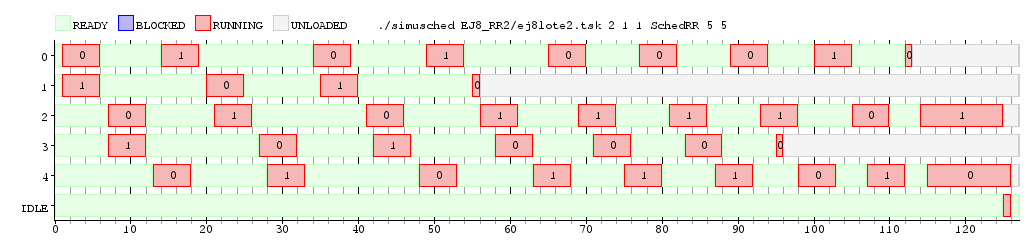
\includegraphics[width=450pt]{./EJ8_RR2/dif10corerr.png}
	{$Lote 3$ - Round Robin - 2 core - Quantum = 5 - cambio de contexto = 1}	
 \end{center}
 
 \begin{center}
    	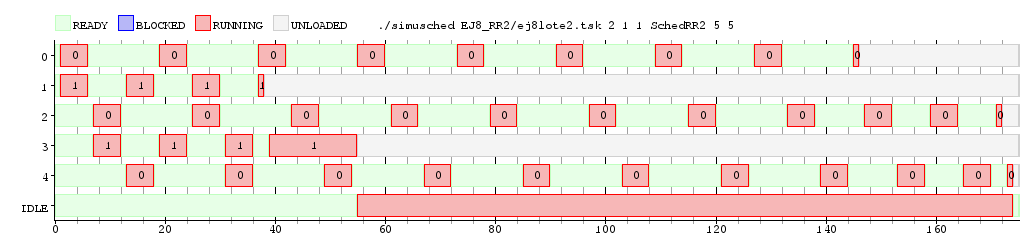
\includegraphics[width=450pt]{./EJ8_RR2/dif10corerr2.png}
	{$Lote 3$ - Round Robin 2 - 2 core - Quantum = 5 - cambio de contexto = 1}	
 \end{center}
 
 Se puede ver en estos diagramas como la implementacion del Round Robin original trabaja
 mejor finalizando la ejecución de las tareas hasta 50 milisegundos antes.\\
 Esto se da por la falta de paralelismo de el RR2 ya que al ser asignados los procesos
 a cada core, cuando uno de los dos finaliza, este queda ocioso ya que no existe la
 posibilidad de migrar  procesos.\\
 
 Por ultimo, nuestra tercer y ultima conjetura:\\
 
 \textbf{Comportamiento mas eficiente en el RR2 con lotes de tareas que se bloquean un gran numero
de veces}

Para esta conjetura, trabajamos con lotes de tareas que utilicen el CPU y se bloqueen muchas
veces para poder demostrar la mejor performance del RR2.\\

A continuacion un ejemplo, con el siguiente lote:

\begin{verbatim}
                                     TaskCPU 40
                                     TaskBatch 10  5
                                     TaskCPU 50
                                     TaskBatch 15 8
                                     TaskCPU 10

\end{verbatim}


   \begin{center}
    	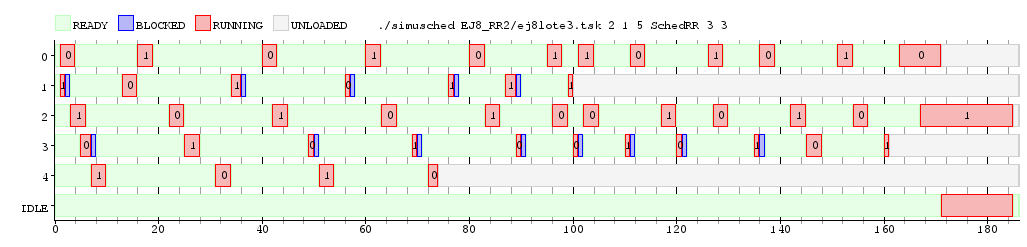
\includegraphics[width=450pt]{./EJ8_RR2/dif5corerr.png}
	{$Lote 3$ - Round Robin - 2 core - Quantum = 3 - cambio de contexto = 1}	
 \end{center}
 
 \begin{center}
    	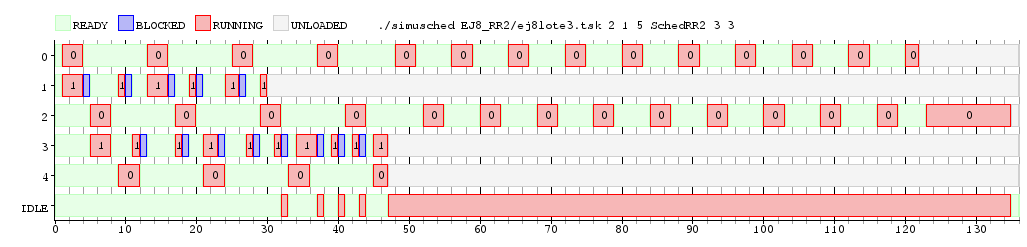
\includegraphics[width=450pt]{./EJ8_RR2/dif5corerr2.png}
	{$Lote 3$ - Round Robin 2 - 2 core - Quantum = 3 - cambio de contexto = 1}	
 \end{center}

 Se puede observar por los diagramas como el RR2 tiene una mejor performance en este estilo
 de lotes llegando a finalizar las ejecuciones hasta 50 milisegundos antes que el Round-Robin
 original.\\
 Como para el Round-Robin original tiene perdida de tiempo con el cambio de contexto y
 migracion de tareas este empeora su performance en comparacion al RR2 que no admite
 este tipo de migracion es notorio la superioridad en relacion a nuestra conjetura.\\
 
 Podemos concluir luego de estas demostraciones que, el Round-Robin original es ampliamente
 superior desde el punto de vista de la performance que obtiene al trabajar con tareas
 que demanden mucho uso del CPU, mientras que el RR2 sera mejor para cuando se utilicen
 tareas que se bloqueen por un tiempo considerable.\\
 
 


  
\subsubsection[Resolución Ejercicio 9]{Ejercicio 9}

\subsubsection[Resolución Ejercicio 10]{Ejercicio 10}
